\documentclass[fontsize=12pt,
               paper=a4,
               twoside=false,
               parskip=half,
               ]{scrartcl}

% Load the packages
%   Copyright 2012 Comet Engineering, Patrick Haring & Christian Bürgi
%
%   Licensed under the Apache License, Version 2.0 (the "License");
%   you may not use this file except in compliance with the License.
%   You may obtain a copy of the License at
%
%       http://www.apache.org/licenses/LICENSE-2.0
%
%   Unless required by applicable law or agreed to in writing, software
%   distributed under the License is distributed on an "AS IS" BASIS,
%   WITHOUT WARRANTIES OR CONDITIONS OF ANY KIND, either express or implied.
%   See the License for the specific language governing permissions and
%   limitations under the License.

% Packages Template
% =================
% 
% Contains packages used for project documentation
% 
% @author burgc5
% 
% To use this simply enter: %   Copyright 2012 Comet Engineering, Patrick Haring & Christian Bürgi
%
%   Licensed under the Apache License, Version 2.0 (the "License");
%   you may not use this file except in compliance with the License.
%   You may obtain a copy of the License at
%
%       http://www.apache.org/licenses/LICENSE-2.0
%
%   Unless required by applicable law or agreed to in writing, software
%   distributed under the License is distributed on an "AS IS" BASIS,
%   WITHOUT WARRANTIES OR CONDITIONS OF ANY KIND, either express or implied.
%   See the License for the specific language governing permissions and
%   limitations under the License.

% Packages Template
% =================
% 
% Contains packages used for project documentation
% 
% @author burgc5
% 
% To use this simply enter: %   Copyright 2012 Comet Engineering, Patrick Haring & Christian Bürgi
%
%   Licensed under the Apache License, Version 2.0 (the "License");
%   you may not use this file except in compliance with the License.
%   You may obtain a copy of the License at
%
%       http://www.apache.org/licenses/LICENSE-2.0
%
%   Unless required by applicable law or agreed to in writing, software
%   distributed under the License is distributed on an "AS IS" BASIS,
%   WITHOUT WARRANTIES OR CONDITIONS OF ANY KIND, either express or implied.
%   See the License for the specific language governing permissions and
%   limitations under the License.

% Packages Template
% =================
% 
% Contains packages used for project documentation
% 
% @author burgc5
% 
% To use this simply enter: \input{./packages.tex}

\usepackage[utf8]{inputenc}
\usepackage[T1]{fontenc}

% Set font to latin modern
\usepackage{lmodern}

\usepackage[pdftex]{graphicx}
\usepackage{epstopdf}

% Create links in pdf documents
\usepackage[colorlinks,pdfpagelabels,pdfstartview=FitH,bookmarksopen=true,bookmarksnumbered=true,linkcolor=black,plainpages=false,hypertexnames=false,citecolor=black] {hyperref}
\hypersetup{
    colorlinks,%
    citecolor=black,%
    filecolor=black,%
    linkcolor=black,%
    urlcolor=black
}
\urlstyle{same}

% Use \enquote{} to create quotation marks
\usepackage{csquotes}

% Create professional tables with booktabs
% @see http://en.wikibooks.org/wiki/LaTeX/Tables#Professional_tables
\usepackage{booktabs}

% Customizable enumerates/itemizes
\usepackage{enumitem}

% git meta information
\usepackage{gitinfo}


\usepackage[utf8]{inputenc}
\usepackage[T1]{fontenc}

% Set font to latin modern
\usepackage{lmodern}

\usepackage[pdftex]{graphicx}
\usepackage{epstopdf}

% Create links in pdf documents
\usepackage[colorlinks,pdfpagelabels,pdfstartview=FitH,bookmarksopen=true,bookmarksnumbered=true,linkcolor=black,plainpages=false,hypertexnames=false,citecolor=black] {hyperref}
\hypersetup{
    colorlinks,%
    citecolor=black,%
    filecolor=black,%
    linkcolor=black,%
    urlcolor=black
}
\urlstyle{same}

% Use \enquote{} to create quotation marks
\usepackage{csquotes}

% Create professional tables with booktabs
% @see http://en.wikibooks.org/wiki/LaTeX/Tables#Professional_tables
\usepackage{booktabs}

% Customizable enumerates/itemizes
\usepackage{enumitem}

% git meta information
\usepackage{gitinfo}


\usepackage[utf8]{inputenc}
\usepackage[T1]{fontenc}

% Set font to latin modern
\usepackage{lmodern}

\usepackage[pdftex]{graphicx}
\usepackage{epstopdf}

% Create links in pdf documents
\usepackage[colorlinks,pdfpagelabels,pdfstartview=FitH,bookmarksopen=true,bookmarksnumbered=true,linkcolor=black,plainpages=false,hypertexnames=false,citecolor=black] {hyperref}
\hypersetup{
    colorlinks,%
    citecolor=black,%
    filecolor=black,%
    linkcolor=black,%
    urlcolor=black
}
\urlstyle{same}

% Use \enquote{} to create quotation marks
\usepackage{csquotes}

% Create professional tables with booktabs
% @see http://en.wikibooks.org/wiki/LaTeX/Tables#Professional_tables
\usepackage{booktabs}

% Customizable enumerates/itemizes
\usepackage{enumitem}

% git meta information
\usepackage{gitinfo}


\begin{document}

% Document title for title.tex
\newcommand{\doctitle}{Use Case Model}
% Titlepage Template
% ==================
% 
% @author burgc5
% 
% To use this simply enter: % Titlepage Template
% ==================
% 
% @author burgc5
% 
% To use this simply enter: % Titlepage Template
% ==================
% 
% @author burgc5
% 
% To use this simply enter: \input{./title.tex}
% 
% You have to define the commands '\doctitle' and '\docrevision' to give the 
% document a title and a revision on its titlepage.
% Do this with the following command:
% \newcommand{\doctitle}{Document title goes here}
%
% SVN:
% ----
% You also have to define the variables:
% \SVN $Date$
% \SVN $Revision$
%
% As executing the following command on the file:
% > svn propset svn:keywords "Date Revision" filename.tex
% 
% This titlepage needs:
% \usepackage[pdftex]{graphicx}
% \usepackage{svn}
%

\begin{titlepage}

\begin{center}

% Team-logo

\includegraphics[width=0.35\textwidth]{./comet-logo.eps}\\[2.5cm]    

% Project title
\textsc{\Large Comet Pinball}\\[2cm]

% Document title
{ \huge \bfseries \doctitle{}}\\[3cm]

% Members/Client
\begin{minipage}{0.45\textwidth}
\begin{flushleft} \large
\emph{Team Members:}\\
Patrick \textsc{Haring}\\
Christian \textsc{Bürgi}
\end{flushleft}
\end{minipage}
\begin{minipage}{0.45\textwidth}
\begin{flushright} \large
\emph{Client:} \\
Jean-Pierre \textsc{Caillot}\\
~
\end{flushright}
\end{minipage}

\vfill

{\large 
Revision hash: \gitAbbrevHash \\[0.2cm]
Commit time: \gitCommitterIsoDate \\[0.2cm]
{\footnotesize \itshape \url{https://github.com/boskoop/comet-pinball/}}}

\end{center}

\end{titlepage}
% 
% You have to define the commands '\doctitle' and '\docrevision' to give the 
% document a title and a revision on its titlepage.
% Do this with the following command:
% \newcommand{\doctitle}{Document title goes here}
%
% SVN:
% ----
% You also have to define the variables:
% \SVN $Date$
% \SVN $Revision$
%
% As executing the following command on the file:
% > svn propset svn:keywords "Date Revision" filename.tex
% 
% This titlepage needs:
% \usepackage[pdftex]{graphicx}
% \usepackage{svn}
%

\begin{titlepage}

\begin{center}

% Team-logo

\includegraphics[width=0.35\textwidth]{./comet-logo.eps}\\[2.5cm]    

% Project title
\textsc{\Large Comet Pinball}\\[2cm]

% Document title
{ \huge \bfseries \doctitle{}}\\[3cm]

% Members/Client
\begin{minipage}{0.45\textwidth}
\begin{flushleft} \large
\emph{Team Members:}\\
Patrick \textsc{Haring}\\
Christian \textsc{Bürgi}
\end{flushleft}
\end{minipage}
\begin{minipage}{0.45\textwidth}
\begin{flushright} \large
\emph{Client:} \\
Jean-Pierre \textsc{Caillot}\\
~
\end{flushright}
\end{minipage}

\vfill

{\large 
Revision hash: \gitAbbrevHash \\[0.2cm]
Commit time: \gitCommitterIsoDate \\[0.2cm]
{\footnotesize \itshape \url{https://github.com/boskoop/comet-pinball/}}}

\end{center}

\end{titlepage}
% 
% You have to define the commands '\doctitle' and '\docrevision' to give the 
% document a title and a revision on its titlepage.
% Do this with the following command:
% \newcommand{\doctitle}{Document title goes here}
%
% SVN:
% ----
% You also have to define the variables:
% \SVN $Date$
% \SVN $Revision$
%
% As executing the following command on the file:
% > svn propset svn:keywords "Date Revision" filename.tex
% 
% This titlepage needs:
% \usepackage[pdftex]{graphicx}
% \usepackage{svn}
%

\begin{titlepage}

\begin{center}

% Team-logo

\includegraphics[width=0.35\textwidth]{./comet-logo.eps}\\[2.5cm]    

% Project title
\textsc{\Large Comet Pinball}\\[2cm]

% Document title
{ \huge \bfseries \doctitle{}}\\[3cm]

% Members/Client
\begin{minipage}{0.45\textwidth}
\begin{flushleft} \large
\emph{Team Members:}\\
Patrick \textsc{Haring}\\
Christian \textsc{Bürgi}
\end{flushleft}
\end{minipage}
\begin{minipage}{0.45\textwidth}
\begin{flushright} \large
\emph{Client:} \\
Jean-Pierre \textsc{Caillot}\\
~
\end{flushright}
\end{minipage}

\vfill

{\large 
Revision hash: \gitAbbrevHash \\[0.2cm]
Commit time: \gitCommitterIsoDate \\[0.2cm]
{\footnotesize \itshape \url{https://github.com/boskoop/comet-pinball/}}}

\end{center}

\end{titlepage}

\tableofcontents

%=======
% ACTORS
%=======

\section{Actors}

\subsection{List of actors}

\begin{tabular}{llp{9cm}}
\toprule
\textbf{Actor} & \textbf{Type} & \textbf{Description} \\ 
\midrule
\emph{Player} & primary & \emph{Player}s run the Comet Pinball on their computer.\\
%\emph{Administrator} & primary & The \emph{administrator} is an employee of the hospital as
%well. He is responsible for the hospital's IT systems to work. He configures
%the system for the \emph{doctor}s to work with. He is not a \emph{doctor}. \\ 
%\emph{OT-Logger} & supporting & The \emph{OT-Logger}s are devices which are used to monitor
%\emph{patient}'s temperatures over a period of time. They can be remotely polled by 
%the system. A device can only be reused after appliance on a \emph{patient} if the device was reset.\\ 
%\emph{Patient} & off-stage & \emph{Patient}s have the monitoring device attached for a period from a few days to a few weeks. \\
%\emph{Email-Server} & supporting & The \emph{email-server} will send the activation code for the first authentication of the \emph{doctor} against the server.

\\ 
\bottomrule 
\end{tabular} 

\subsection{Primary actor goals}

\begin{description}

\item[Player:] \hfill \\
A \emph{Player} uses the Comet Pinball to pass his leisure time and enjoy himself. He is interested in a well designed play field with nice visual and acoustical effects.

%\item[Administrator:] \hfill \\
%The \emph{administrator} wants to create and delete accounts for the \emph{doctor}s.

\end{description}

%==================
% Use cases (brief)
%==================


\section{Use cases (brief)}

\subsection{Player}

\begin{description}

\item[Start simulation:]   The player wants to start a game so he enters the main screen of the application and selects the option for starting a new game. The simulator loads the play field, resets the score counter and sets the right amount of available balls for this game and loads one ball in the plunger.

\item[Start game:] The plunger has to be operated to forward the ball onto the play field.  The force can be controlled by some matter.

\item[Move flippers:] The player can move the flippers to prevent the ball from leaving the play field. If the ball is hit by the flippers he follows approximately the movements of a collision.

\item[Ball leaves via drain:] The ball is passing the flippers and leaves the play field via the drain. The simulator loads a new ball in the plunger and decreases the counter of available balls by one.

\item[Extra ball:] 
to do

\item[Extra game:]
to do

\item[Gameover:] All balls have left the play field so the game is over. The score is presented to the user and the user has to start a new game to play further.

\item[Hit obstacle:] The application actualizes the score If a scoring obstacle  was hit. The ball is following the movement of a collision.

\item[Stuck ball:] The ball is stuck somewhere on the play field, so the user has the possibility to tilt the table.

\item[Tilt:] If the play field was tilted too often or too hard, the game will stop and display the user the message "Tilt".

\item[New Highscore:] If a game is over and the score has exceeded the highscore, the application will produce visual and acoustic effects. The score will be set as new highscore and the new highscore sheet is presented to the player.

\item[Watch Highscores:] 
to do

\item[Configure game properties:] The properties of the game like size of the bumpers, amount of available balls and other settings can be configured in a properties file.

\end{description}


%==========================
% Use cases (fully-dressed)
%==========================


%==========================
% UC1
%==========================

\section{Use cases (fully-dressed)}

\subsection{Use Case UC1: Start simulation}

\textbf{\textsf{Scope:}} Comet Pinball

\textbf{\textsf{Level:}} user goal

\textbf{\textsf{Primary actor:}} \emph{Player}

\textbf{\textsf{Preconditions:}} \emph{Player} has started the application on his Computer and has arrived on the main screen.

\textbf{\textsf{Postconditions:}} The name of the \emph{Player} has been entered, the plunger is filled with a ball and all counters are reset.

\textbf{\textsf{Main success scenario:}}

\begin{enumerate}[leftmargin=3em]
	\item \emph{Player} initiates the start of the simulation.
	\item Application is starting the simulation with the \emph{Player}'s nickname.
	\item Application sets the counter of the available balls to default value
	\item Application sets the score to zero.
	\item Application activates the plunger and puts one ball in it. 
	\item Application activates the flippers.
\end{enumerate}


\begin{itemize}[leftmargin=3em]
	\item[2a.] 	\emph{Player} has not yet entered his nickname.
	\begin{enumerate}
		\item Application prompts for the \emph{Player}'s nickname.
		\item \emph{Player} enters his nickname.
		\item Application stores the nickname.
	\end{enumerate}
\end{itemize}


%==========================
% UC2
%==========================

\section{Use cases (fully-dressed)}

\subsection{Use Case UC2: Start Game}

\textbf{\textsf{Scope:}} Comet Pinball

\textbf{\textsf{Level:}} user goal

\textbf{\textsf{Primary actor:}} \emph{Player}

\textbf{\textsf{Preconditions:}} \emph{Player} has started a simulation.

\textbf{\textsf{Postconditions:}} The ball has entered the play field and the game has started.

\textbf{\textsf{Main success scenario:}}

\begin{enumerate}[leftmargin=3em]
	\item \emph{Player} is applying the plunger and adds some force to the ball.
	\item Application simulates the ball's movement.
	\item The ball enters play field.
\end{enumerate}


\begin{itemize}[leftmargin=3em]
	\item[3a.] Ball has not enough force to climb the ramp and rolls back into the plunger.
	\begin{enumerate}
		\item Continue with 1.
	\end{enumerate}
\end{itemize}



%==========================
% UC3
%==========================

\section{Use cases (fully-dressed)}

\subsection{Use Case UC3: Move flippers}

\textbf{\textsf{Scope:}} Comet Pinball

\textbf{\textsf{Level:}} user goal

\textbf{\textsf{Primary actor:}} \emph{Player}

\textbf{\textsf{Preconditions:}} \emph{Player} has started a simulation.

\textbf{\textsf{Postconditions:}} The ball has entered the play field and the game has started.

\textbf{\textsf{Main success scenario:}}

\begin{enumerate}[leftmargin=3em]
	\item \emph{Player} example
\end{enumerate}


\begin{itemize}[leftmargin=3em]
	\item[*a.] example
	\begin{enumerate}
		\item example
	\end{enumerate}
\end{itemize}



\section{Use case diagram}


% Diagram generated with astah
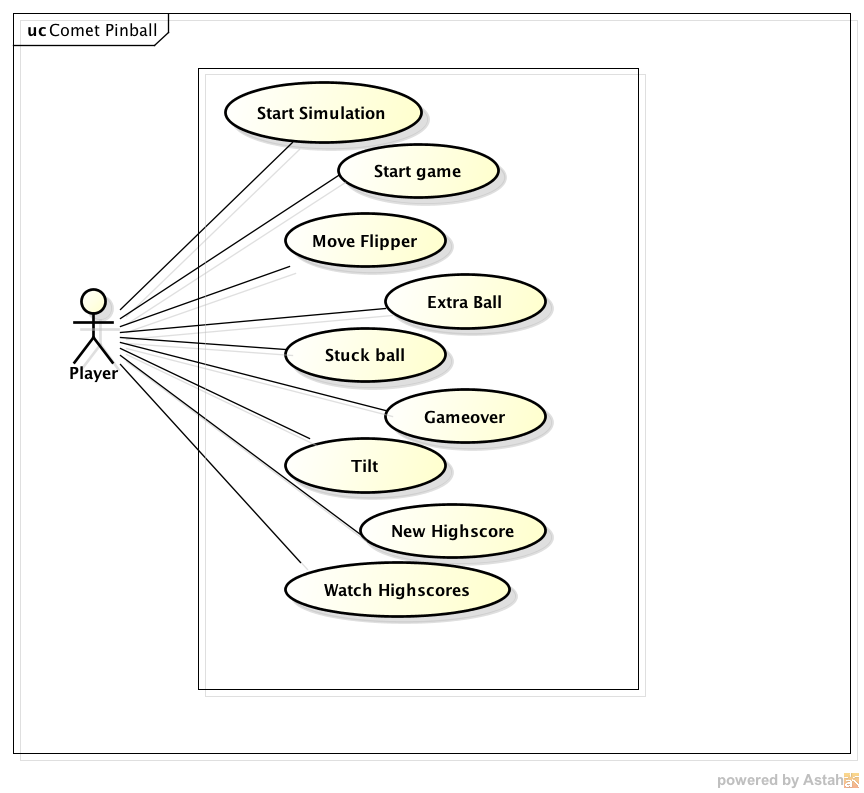
\includegraphics[width=15cm]{./img/usecase-model.png}

\end{document}